%%%%%%%%%%%%%%%%%%%%%%%%%%%%%%%%%%%%%%%%%%%%%%%%%%%%%%%%%%%%%%%%%%%%%%%%%%%%%%%%%%%%%%%%%
%%                                                                                     %%
%%                This file is part of the CAPH Compiler distribution                  %%
%%                            http:%/caph.univ-bpclermont.fr                           %%
%%                                                                                     %%
%%                                  Jocelyn SEROT                                      %%
%%                         Jocelyn.Serot@univ-bpclermont.fr                            %%
%%                                                                                     %%
%%         Copyright 2011-2018 Jocelyn SEROT.  All rights reserved.                    %%
%%  This file is distributed under the terms of the GNU Library General Public License %%
%%      with the special exception on linking described in file ..%LICENSE.            %%
%%                                                                                     %%
%%%%%%%%%%%%%%%%%%%%%%%%%%%%%%%%%%%%%%%%%%%%%%%%%%%%%%%%%%%%%%%%%%%%%%%%%%%%%%%%%%%%%%%%%

\chapter{Working with projects}
\label{cha:ide-project}

The \caph IDE provides a simple way of organizing files related to a given application within an entity
called a \emph{project}. Technically, a \emph{project} is nothing but a directory gathering all
files related to an application. This includes \caph source files, input data files for simulation,
files saving compiler options and a collection of subdirectories containing the files
produced by the compiler in graph, simulation, SystemC or VHDL mode. Having a separate directory for
each mode makes interfacing to external tools -- C++ compiler, VHDL simulators and synthetizers in
particular -- easier.

\medskip
In this chapter we will describe first how to create new projects and second how to use existing projects.

\section{Creating a project}
\label{sec:creating-project}

For simplicity, the created project will include a single source file, similar to that used
in chapter~\ref{cha:ide-basic}.

\medskip
\step \textbf{Create a new project} by invoking the corresponding item in the \textsf{File}
menu. In the displayed dialog (Fig.~\ref{fig:create-project}) give a a name to the project and
specify a directory to host it. For example, if the name is \texttt{myproj} and the root directory
\verb|C:\Users\Bob\Desktop|, then all the files related to the project will be stored in
directory \verb|C:\Users\Bob\Desktop\myproj|. If the projet needs additionnal, pre-existing
source or data files, add them in the corresponding text box or using the provided button. These
files will be automatically copied in the project directory. No additionnal file is needed here.

\begin{figure}[h]
  \centering
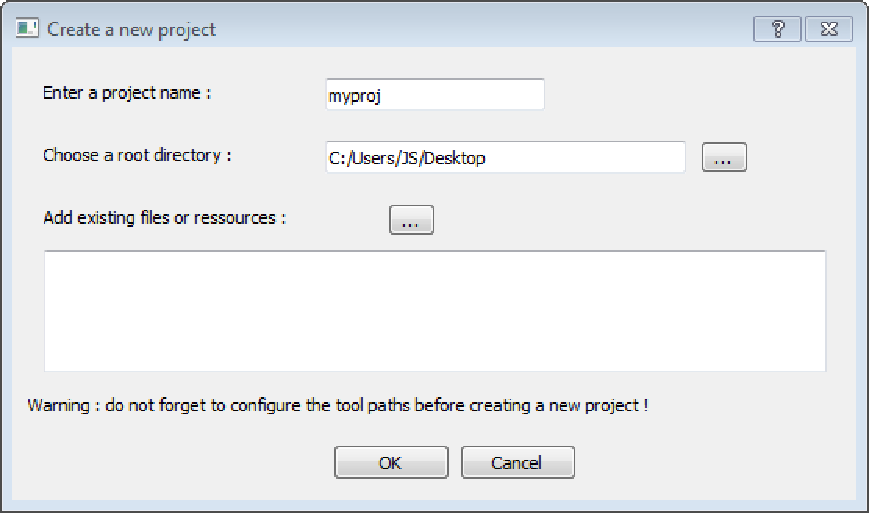
\includegraphics[width=0.75\textwidth]{figs/ide/create-project}
  \caption{The dialog shown when creating a new project}
  \label{fig:create-project}
\end{figure}

\step When a project \texttt{myproj} is created, a "main" source file is created with name
\texttt{main.cph} in the project directory and a file tab for editing is file is created (see
Fig.~\ref{fig:project-main}). Type the \caph source code of your program here\footnote{If you
  already have the source code, you can of course copy it and paste it.} and save it (see
Fig.~\ref{fig:project-main-done}). 

\begin{figure}[h]
  \centering
  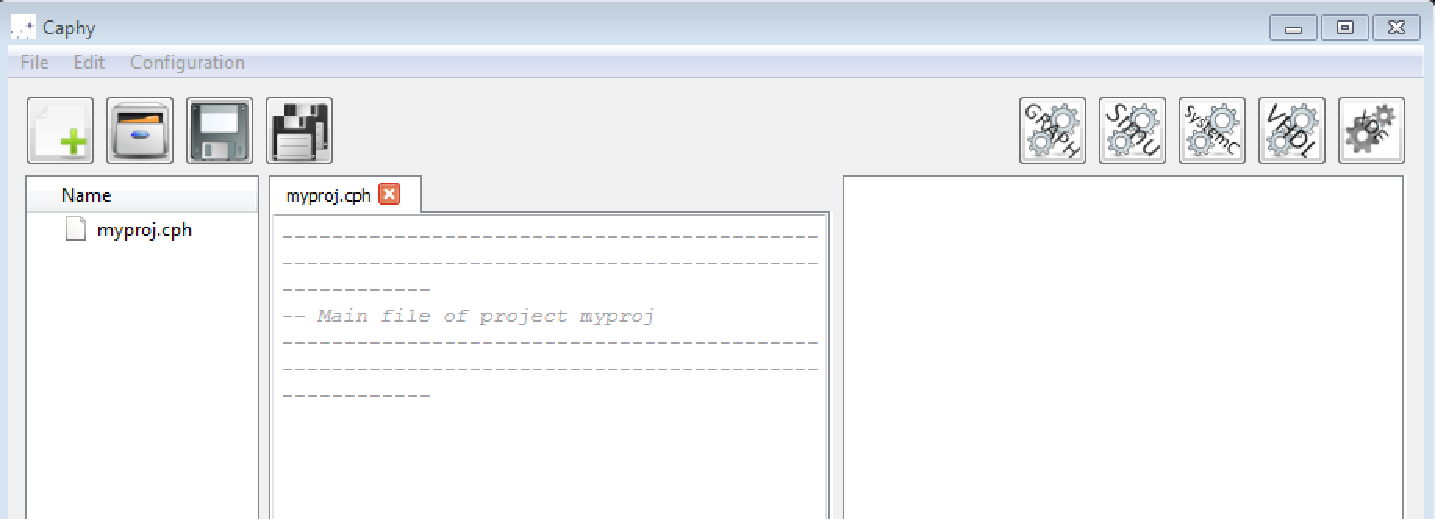
\includegraphics[width=0.75\textwidth]{figs/ide/project-main}
  \caption{Ready to edit the project main source file}
  \label{fig:project-main}
\end{figure}

\begin{figure}[h]
  \centering
  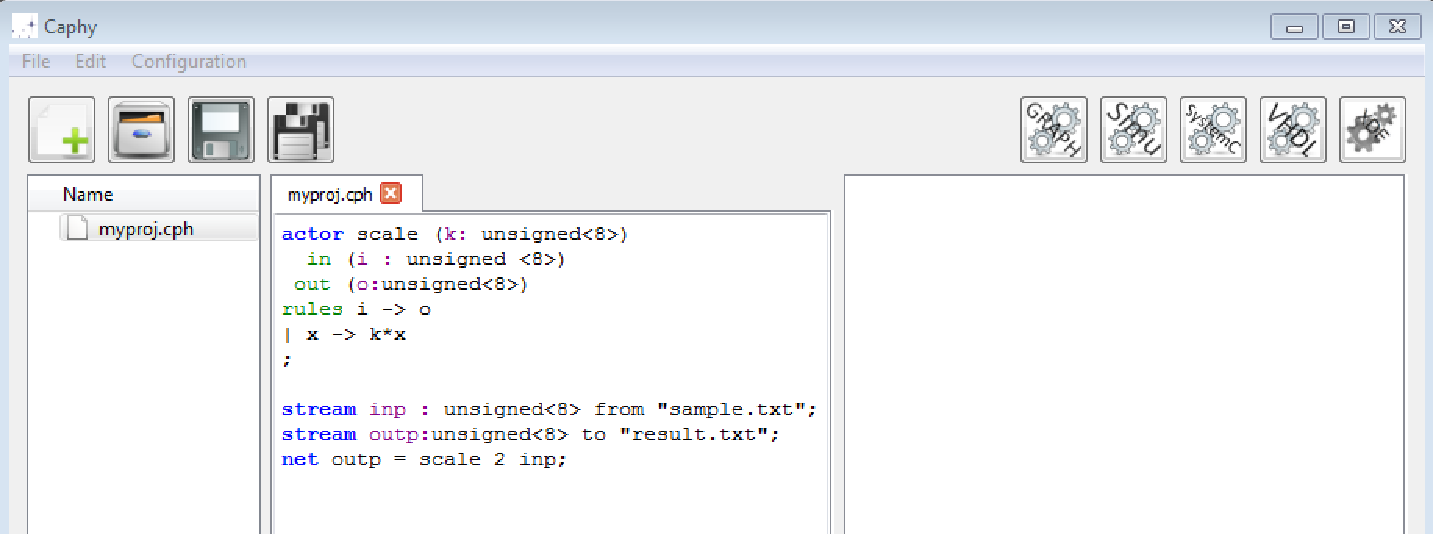
\includegraphics[width=0.75\textwidth]{figs/ide/project-main-done}
  \caption{Main source file completed}
  \label{fig:project-main-done}
\end{figure}

\medskip
\step From now, each compile action will 
\begin{itemize}
\item implicitely operate on the project main source file,
\item generate results in a specific directory (\texttt{dot} for graph, \texttt{simu} for
  simulation, \texttt{systemc}, \texttt{vhdl} and \texttt{xdf}).
\end{itemize}

The project tree representation (on the left) will be automatically updated to reflect the effect of
each compile action. Navigation within this tree  is of course allowed and double clicking on an
element will open the corresponding file in a distinct tab (if not already opened).

For example, Fig.~\ref{fig:project-make} display the GUI after clicking the \textsf{Graph}
and the \textsf{SystemC} compile buttons. The complete list of generated files for each step can be viewed by
clicking on the respective subdirectory in the tree view on the left.

\begin{figure}[h]
  \centering
  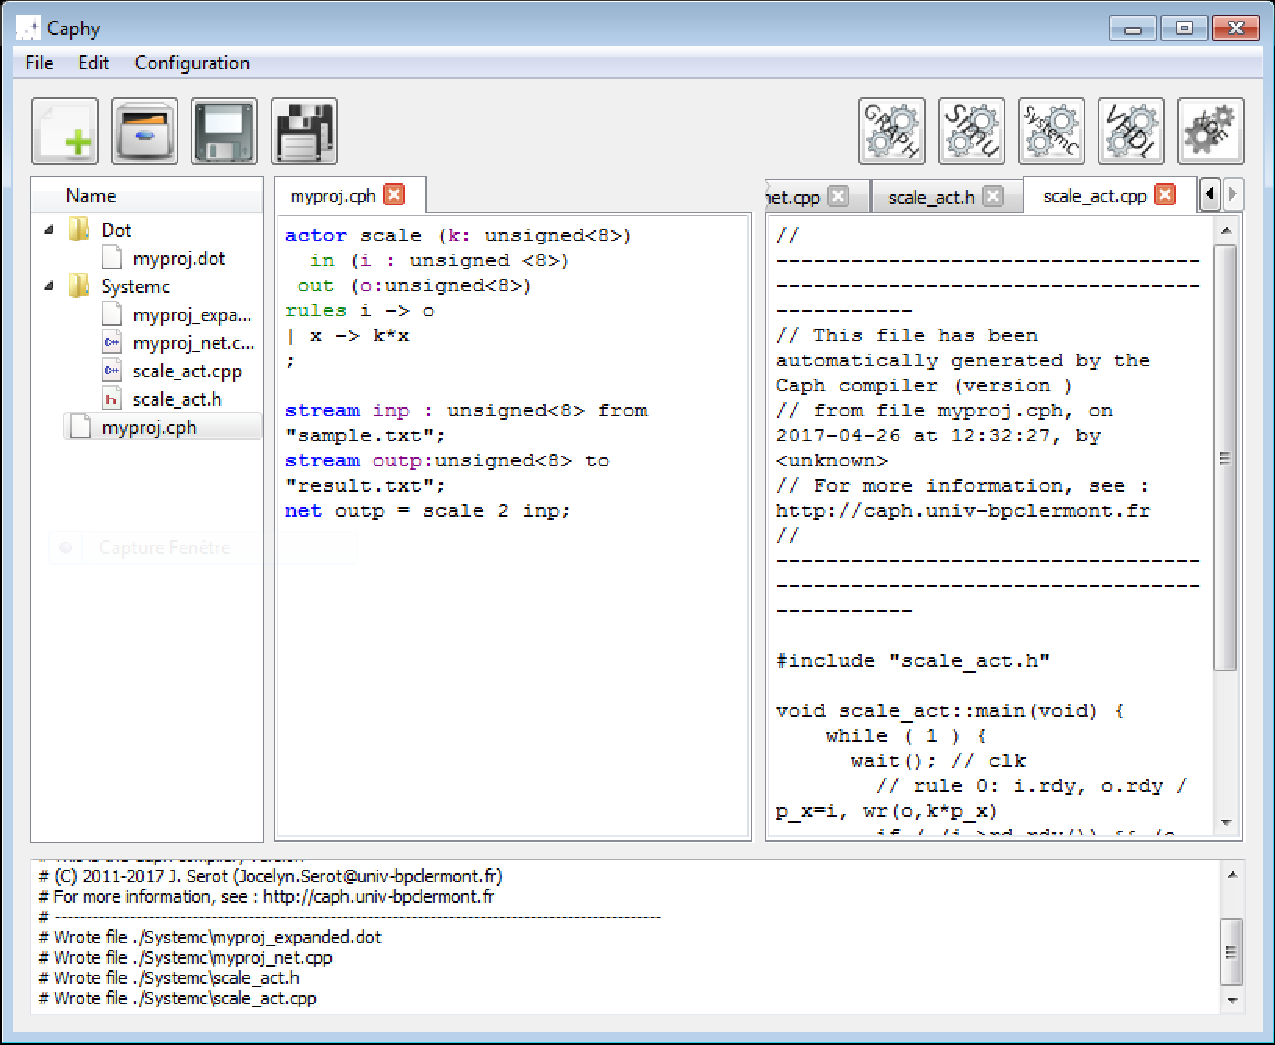
\includegraphics[width=0.75\textwidth]{figs/ide/project-make}
  \caption{After clicking the \textsf{Graph} and \textsf{SystemC} buttons in project mode}
  \label{fig:project-make}
\end{figure}

% \begin{figure}[h]
%   \centering
%   %\includegraphics[width=0.75\textwidth]{figs/first-launch}
%   \caption{After clicking the \textsf{SystemC} button in project mode}
%   \label{fig:project-make-sysc}
% \end{figure}

\section{Opening an existing project}
\label{sec:opening-a-project}

To open an existing projec, invoke the \textsf{Open Project} item of the
\textsf{File} menu and specify the name of the project description file (ending with the
\verb|.cphpro| extension), located in the project directory.

\medskip
For example, Fig.~\ref{fig:opening-primer-proj} shows the IDE
just about to open the project located in \texttt{primer/simple} directory which can be found in the
examples provided with the \caph distribution\footnote{These examples have here been installed in
  \texttt{Documents/CaphExamples}.}. This project corresponds to the program described in Part 1 of
this document. 

Fig.~\ref{fig:opened-primer-proj} shows the IDE just after opening this project.
 
\begin{figure}[h]
  \centering
  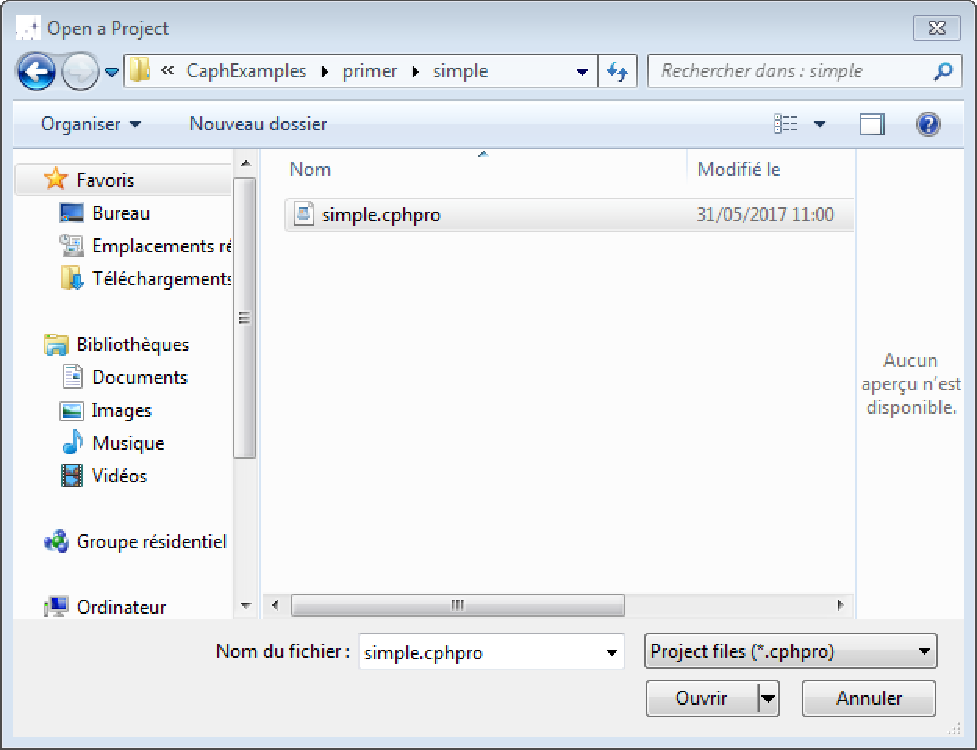
\includegraphics[width=0.75\textwidth]{figs/ide/opening-project}
  \caption{About to open the \texttt{Primer} project}
  \label{fig:opening-primer-proj}
\end{figure}

\begin{figure}[h]
  \centering
  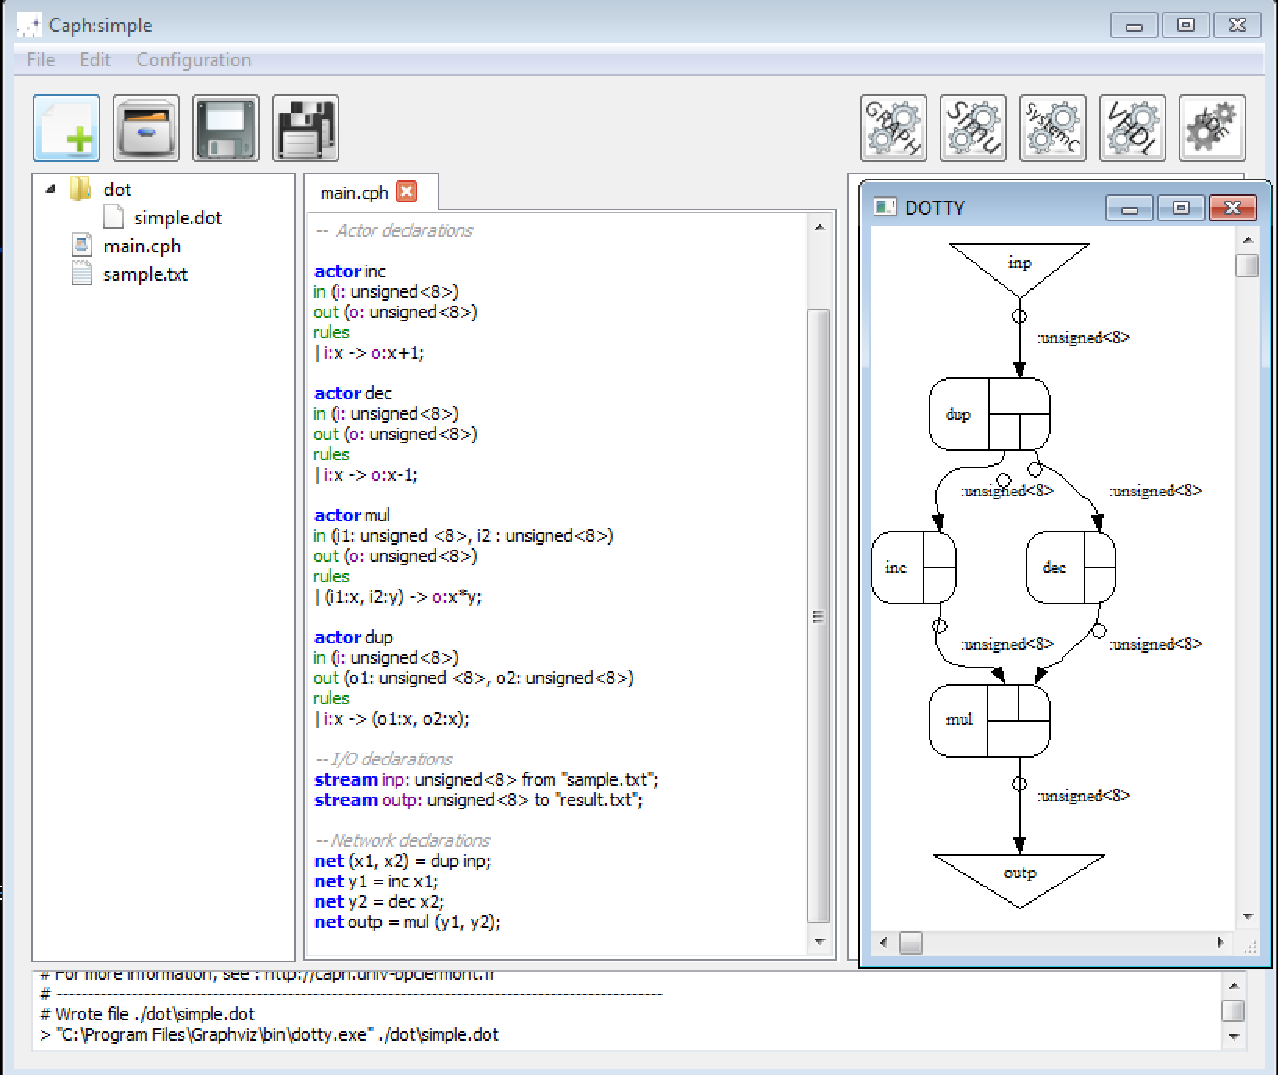
\includegraphics[width=0.95\textwidth]{figs/ide/opened-project}
  \caption{The \texttt{Primer} project opened}
  \label{fig:opened-primer-proj}
\end{figure}

%%% Local Variables: 
%%% mode: latex
%%% TeX-master: "caph-primer"
%%% End: 
